%Part of/Parte di https://github.com/f-dinucci/appuntiMeccanicaFluidi/
%License/Licenza Creative Commons Attribution-ShareAlike 4.0 International (CC BY-SA 4.0) - attribution/attribuzione Francesco Di Nucci
%See also/Vedere anche https://creativecommons.org/licenses/by-sa/4.0/ and/e https://creativecommons.org/licenses/by-sa/4.0/legalcode
%
\section{Equazioni del moto turbolento}  
Si è visto che in certe condizioni il moto è turbolento, cioè agitato anche nel caso in cui ci si aspetterebbe un moto stazionario, per motivi legati a viscosità e numero di Reynolds.
È difficile da simulare al calcolatore, dato che la potenza di calcolo necessaria aumenta col cubo del numero di Reynolds, e non vi sono soluzioni matematiche esatte, si preferisce quindi ragionare su grandezze medie per semplificare i calcoli.

%SUBSECTION
\subsection{Richiami di statistica}
Data una $u(x,t)$ se ne può fare la media in modi differenti, effettuando un solo esperimento e vedendo le variazioni nel tempo (media temporale) o effettuando $n$ esperimenti e mediando i risultati:
%
	\begin{equation*}
		\begin{gathered}
			\text{media temporale} \quad \frac{1}{t}\int_o^T u(x,t) \dd{t}\\
			\text{media di insieme} \quad \frac{1}{N} \sum_n u_n(x,i)
		\end{gathered}
	\end{equation*}
%
la media d'insieme praticamente si usa solo a livello concettuale, ma nel caso il fenomeno cambi nel tempo non può essere utilizzata la media temporale.
Nel caso le due medie siano uguali il problema è detto ergodico (la proprietà è detta ergodicità).

L'operazione di media è lineare:
%
	\begin{equation*}
		\begin{gathered}
			<u_1 + u_2> = <u_1> + <u_2>\\
			<a u_1 + b u_2> = a <u_1> + b <u_2>
		\end{gathered}
	\end{equation*}
%
È quindi possibile definire un rapporto incrementale:
%
	\begin{equation*}
		\left< \frac{u(t + \Delta t, x) - u(t,x)}{\Delta t} \right> = \frac{<u(t + \Delta t, x)> - <u(t,x)>}{\Delta t}
	\end{equation*}
%
Al limite:
%
	\begin{equation*}
		\begin{gathered}
			\left< \pdv{u}{t} \right> = \pdv{<u>}{t}\\
			\left< \pdv{u}{x} \right> = \pdv{<u>}{x}
		\end{gathered}
	\end{equation*}
%

%SUBSECTION
\subsection{Equazioni del moto}
Quindi l'equazione di continuità diventa:
%
	\begin{equation*}
		\left< \pdv{u}{x} + \pdv{v}{y} + \pdv{w}{z} \right> = \pdv{<u>}{x} + \pdv{<v>}{y} + \pdv{<w>}{t} = 0
	\end{equation*}
%

Il problema sono le equazioni per la quantità di moto, che hanno termini non lineari, ad esempio
%
	\begin{equation*}
		<uv> \neq <u> <v>
	\end{equation*}
%
Si definiscono le fluttuazioni come scostamenti dalla media, $u' = u - <u>$, quindi:
%
	\begin{equation*}
		\begin{gathered}
			<(<u> + u') (<v> + v') > = \\
			= <<u> + <v>> + <u' <v> > + < <u> v' > + < u' v' > =
		\end{gathered}
	\end{equation*}
%
Dato che la media di una fluttuazione è nulla, che la media di una costante è la costante stessa e che le medie sono costanti ($< <u> <v>  > = < u > < v >$):
%
	\begin{equation*}
		= <u> <v> + \cancel{<u'> <v>} + \cancel{<u> <v'>} + <u' v'>
	\end{equation*}
%
Alla fine:
%
	\begin{equation*}
		\begin{gathered}
			<uv> = <u> <v> + <u' v'>\\
			<\uline{v} \uline{v}> = <\uline{v}> <\uline{v}> + <\uline{v}' \uline{v}'>
		\end{gathered}
	\end{equation*}
%

Quindi per la quantità di moto, partendo dalla forma conservativa:
%
	\begin{equation*}
		\begin{gathered}
			\pdv{\uline{v}}{t} + \div{(\uline{v} \uline{v})} + \frac{1}{\rho} \grad{p} = \nu \laplacian{ \uline{v} }\\
			\pdv{<\uline{v}>}{t} + \div{<\uline{v} \uline{v}>} + \frac{1}{\rho} \grad{<p>} = \nu \laplacian{<\uline{v}>}\\
			\pdv{<\uline{v}>}{t} + \div{(<\uline{v}> <\uline{v}>)} + \div{<\uline{v}' \uline{v}'>} + \frac{1}{\rho} \grad{<p>} = \nu \laplacian{<\uline{v}>}
		\end{gathered}
	\end{equation*}
%
Si è quindi arrivati alle cosiddette \textbf{equazioni mediate di Reynolds}:
%
	\begin{equation*}
		\begin{gathered}
			\left< \pdv{u}{x} + \pdv{v}{y} + \pdv{w}{z} \right> = \pdv{<u>}{x} + \pdv{<v>}{y} + \pdv{<w>}{t} = 0\\
			\pdv{<\uline{v}>}{t} + \div{(<\uline{v}> <\uline{v}>)} + \div{<\uline{v}' \uline{v}'>} + \frac{1}{\rho} \grad{<p>} = \nu \laplacian{<\uline{v}>}
		\end{gathered}
	\end{equation*}
%
Il problema, detto della chiusura, è trovare il tensore degli sforzi di Reynolds: $\uuline{T}_R = \rho <\uline{v'} \uline{v'}>$

%SUBSECTION
\subsection{Moto turbolento in condotto}
 %
	\begin{figure}[ht]
		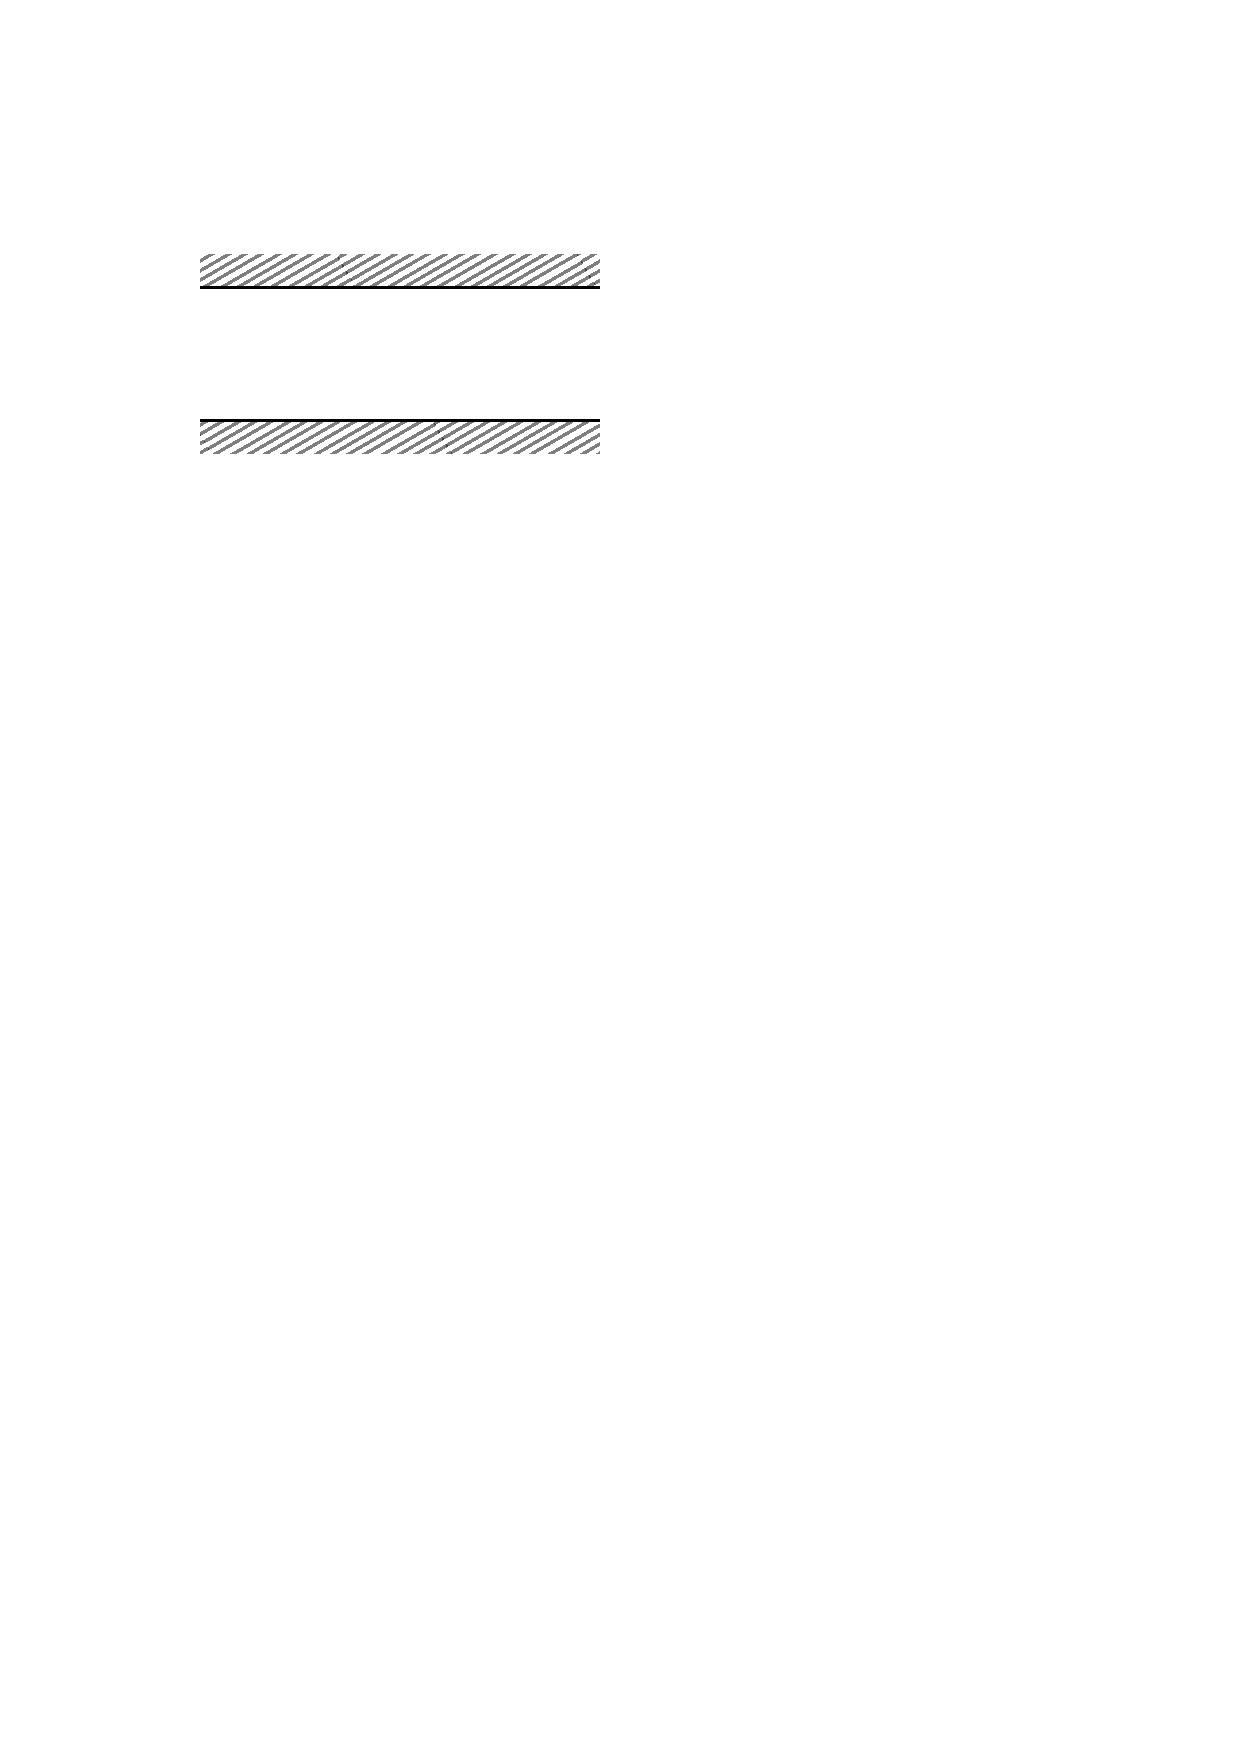
\includegraphics[scale=0.6]{./8.2 Equazioni del moto turbolento/8.2-1}
		\centering
		\caption{Condotto con pareti parallele}
	\end{figure}
%
Dato che si è in un condotto:
%
	\begin{equation*}
		\pdv{t} = \pdv{x} = \pdv{z} = 0
	\end{equation*}
%
Poi nel caso turbolento, per velocità medie e sforzi di Reynolds:
%
	\begin{equation*}
		\cancel{\pdv{\bar{u}}{x}} + \pdv{\bar{v}}{y} + \cancel{\pdv{\bar{w}}{z}} = 0
	\end{equation*}
%

Quindi
%
	\begin{equation*}
		\begin{gathered}
			\cancel{\pdv{\bar{v}}{t}} + \cancel{\div{<\uline{v} \uline{v}>}} + \frac{1}{\rho} \div{\uuline{T}_R} + \frac{1}{\rho} \grad{\bar{p}} = \nu \pdv[2]{\bar{v}}{y}\\
			\text{presa una componente sola}\\
			\frac{1}{\rho} \left( \cancel{\pdv{T_{Rxx}}{x}} + \pdv{T_{Rxy}}{y}+ \cancel{\pdv{T_{Rxz}}{z}} \right) + \frac{1}{\rho} \pdv{\bar{p}}{x} = \nu \pdv[2]{\bar{u}}{y}
		\end{gathered}
	\end{equation*}
%
Detto quindi $\pdv{\tau_{Rxy}}{y} = \pdv{\tau_R}{y}$, sottintendendo si tratti di medie e riordinando:
%
	\begin{equation*}
			\pdv{\tau_R}{y} + \pdv{p}{x} = - \mu \pdv[2]{u}{y}
	\end{equation*}
%
Integrando l'equazione di cui prima e considerando anche le altre componenti:
%
	\begin{equation*}
		\begin{gathered}
			\pdv{p}{x} = cost.\\
			\tau_R + y \pdv{p}{x} = \mu \pdv{u}{y} + C
		\end{gathered}
	\end{equation*}
%
Da questo si ottiene:
%
	\begin{equation*}
		\begin{gathered}
			\tau_R - \mu \pdv{u}{y} = C - y \pdv{p}{x}\\
			\tau_R \quad \text{sforzo di Reynolds}\\
			- \mu \pdv{u}{y} \quad \text{sforzo viscoso}\\
			C - y \pdv{p}{x} \quad \text{sforzo totale}
		\end{gathered}
	\end{equation*}
%
È possibile tracciare il profilo dello sforzo totale dato che è una retta.
Si riprende poi la definizione di sforzo di Reynolds
%
	\begin{equation*}
		\tau_r = \rho<u' v'>
	\end{equation*}
%
Alla parete non ci sono fluttuazioni, quindi lo sforzo di Reynolds è nullo e lo sforzo totale coincide con lo sforzo viscoso.
Allontanandosi dalla parete invece lo sforzo viscoso diviene trascurabile e lo sforzo totale coincide con lo sforzo di Reynolds.
Si può quindi tracciare un diagramma qualitativo dello sforzo.
 %
	\begin{figure}[ht]
		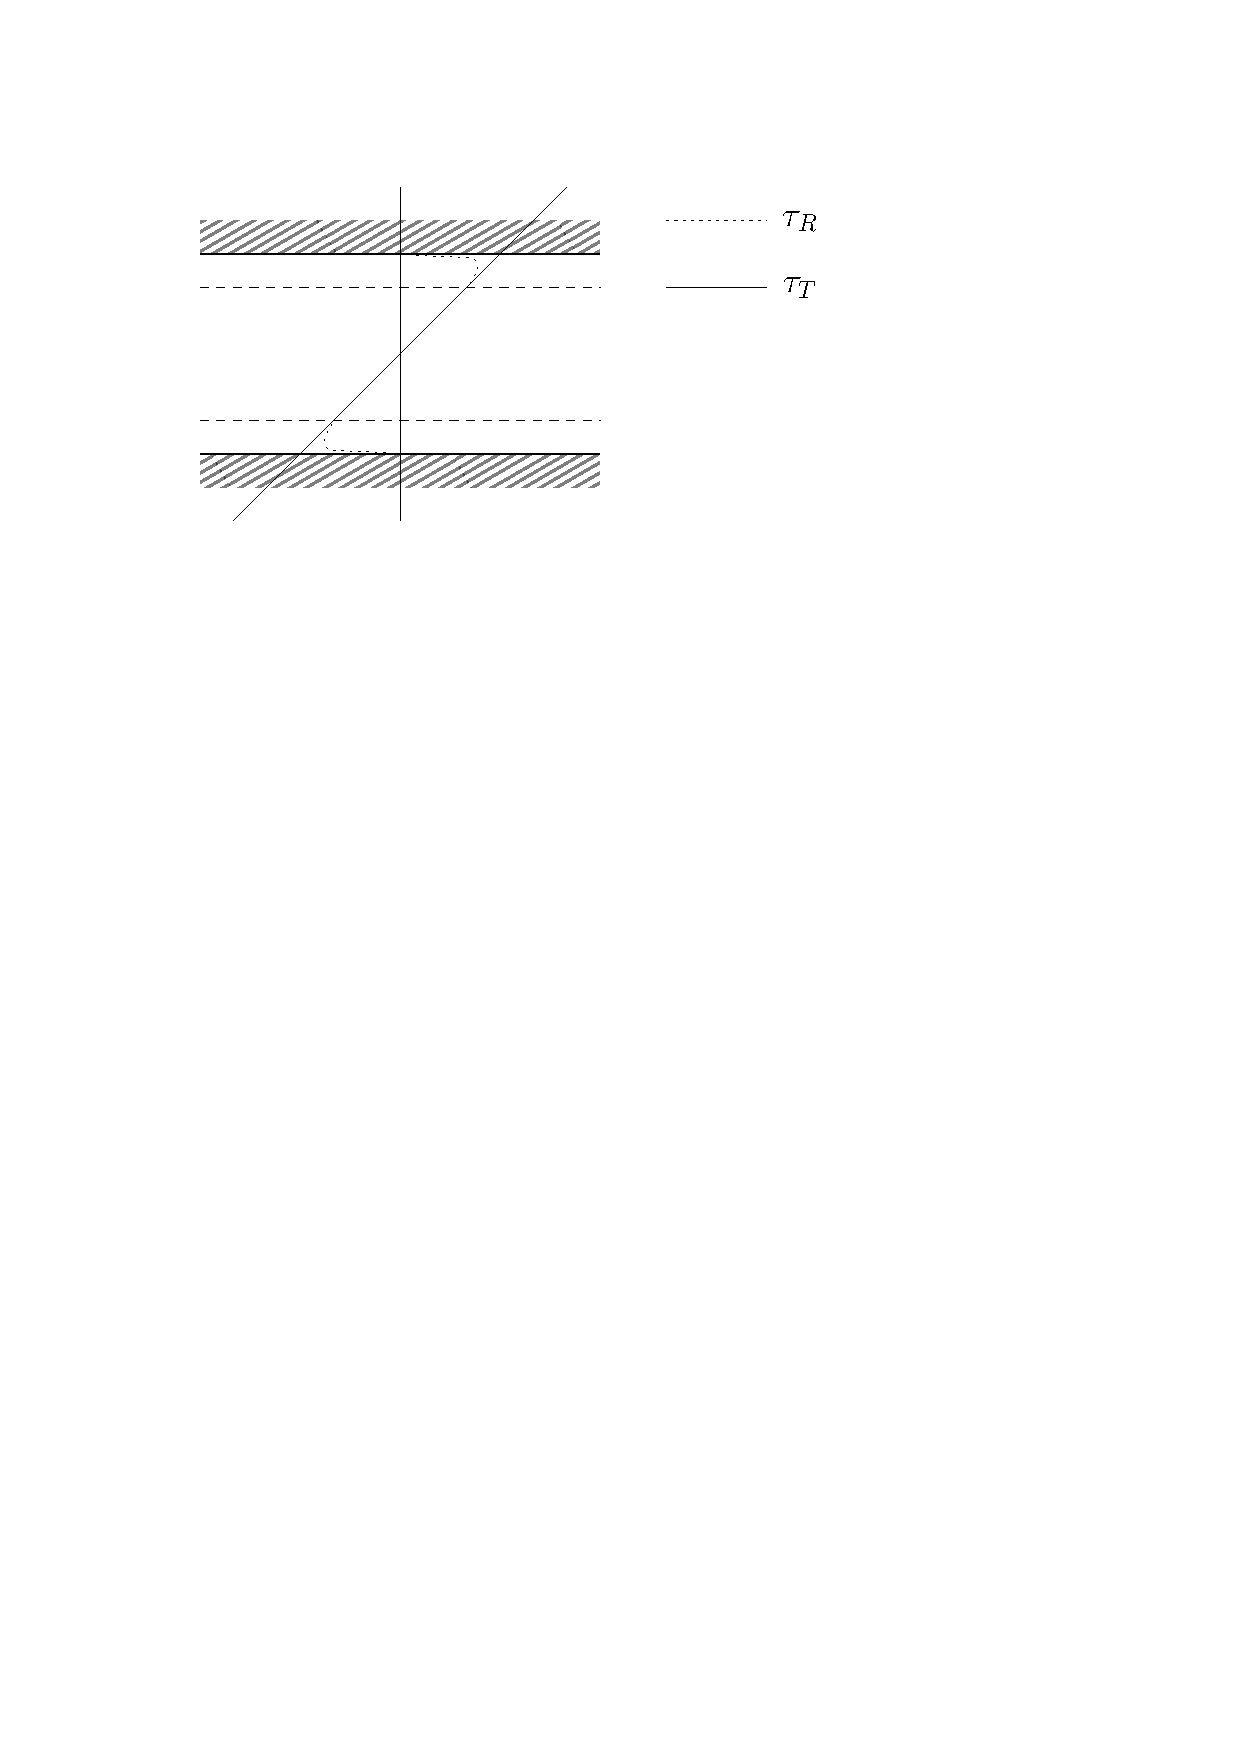
\includegraphics[scale=0.9]{./8.2 Equazioni del moto turbolento/8.2-2}
		\centering
		\caption{Profilo dello sforzo}
	\end{figure}
% 

Per i differenti comportamenti vengono assegnati dei nomi agli strati:
 %
	\begin{figure}[ht]
		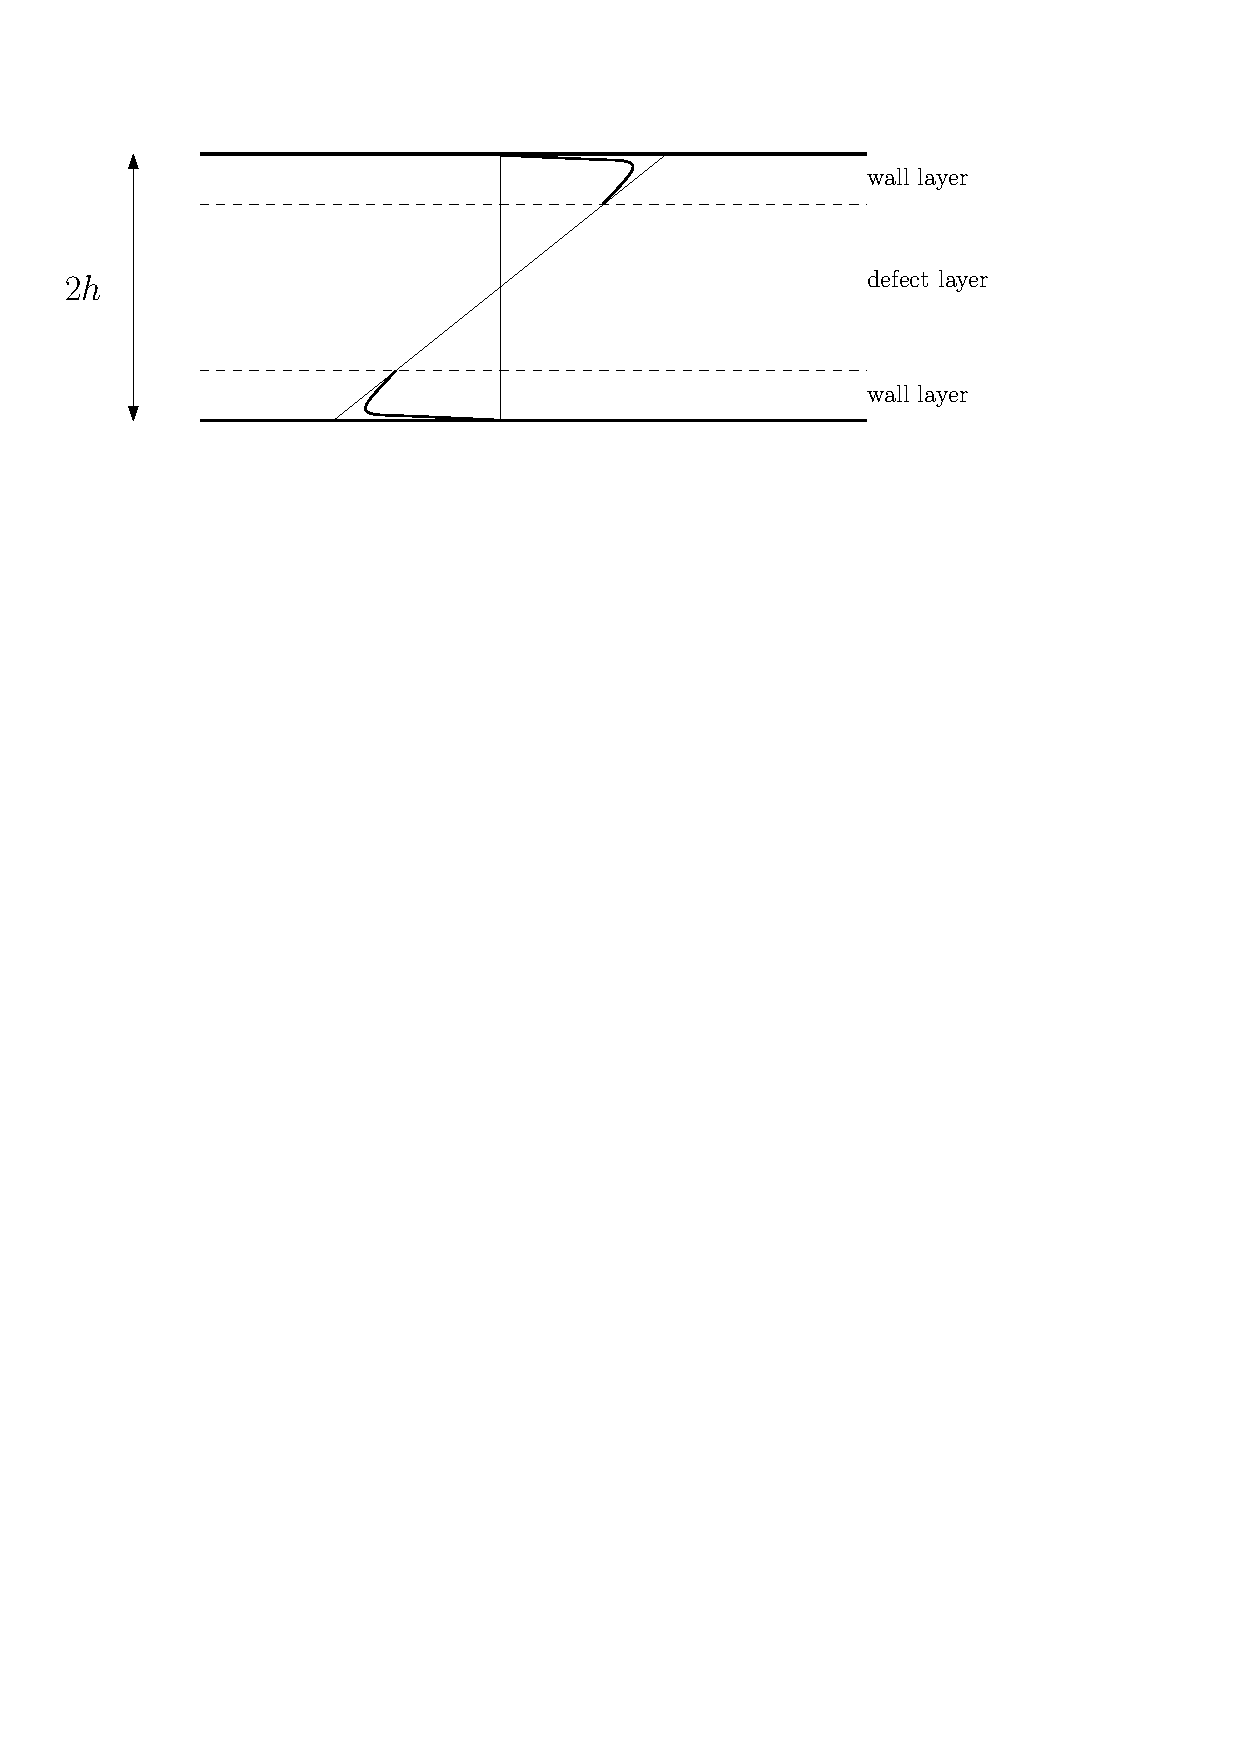
\includegraphics[scale=0.6]{./8.2 Equazioni del moto turbolento/8.2-3}
		\centering
		\caption{Grafico qualitativo dello sforzo}
	\end{figure}
%


\subsection*{Bibliografia 8.2}
\cite[Cap.\ 12.3]{PnueliGutfinger}